% Titre

\makeatletter	% permet d'utiliser les commandes \@ pour reprendre les données du fichier metadata.tex
	\begin{titlepage}

		\begin{figure}[H]
			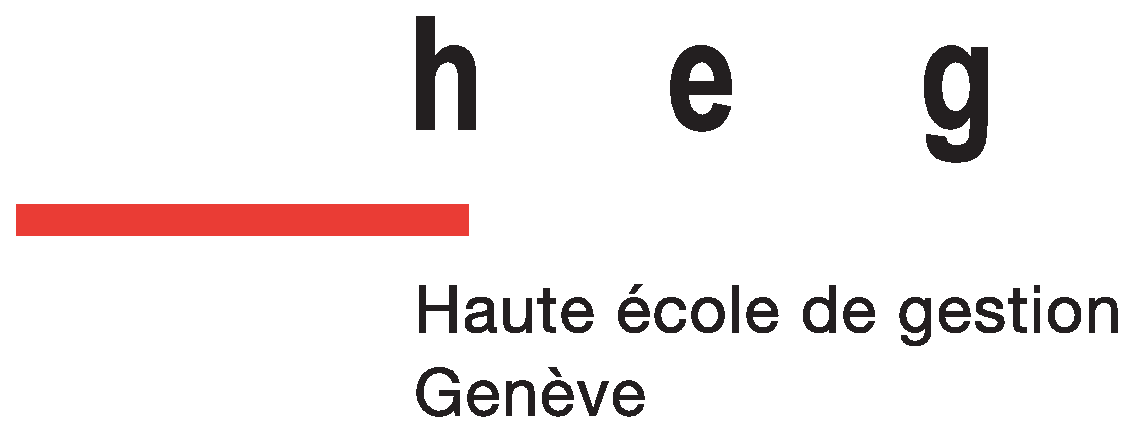
\includegraphics[width=5cm]{images/heg-logo.eps}
		\end{figure}
	
		\begin{center}
			
			{\LARGE \textbf{\@title}} \\

			\vspace{1cm}
			
			<Logo de l'entreprise, si désiré>\\	% supprimer les lignes non nécessaires le cas échéant
			
			\vspace{.2cm}
			
			
\includegraphics[width=2cm]{images/logo-mandant.png}
			
			\vspace{1cm}
			\vfill
		
			{\large < S'IL Y A LIEU, ajouter la mention suivante >}
				\textbf{\Large{ \textsc{ \underline{< Travail strictement confidentiel >}}}}\\

			\vspace{2cm}

			\textbf{Travail de <Bachelor/Master> réalisé en vue de l’obtention du <Bachelor/Master> HES}\\
				par\textbf{\,}:\\
				{\large \@author} \\

			\vspace{1cm}
      \vfill

			Conseiller au travail de <Bachelor / Master>\,:\\
				\textbf{\Large{} <Prénom> \textsc{<Nom>}, <titre de la personne>}\\

			\vspace{2cm}
			\vfill		

			\textbf{\large <Lieu>, \today{}}\\
				\textbf{\large Haute École de Gestion de Genève (HEG-GE)}\\
				\textbf{\large <filière>}\\

		\end{center}

 		\vfill
		
			\begin{flushright}
		 		
\includegraphics[width=4cm]{images/hes-logo.eps}
			\end{flushright}
  
	\end{titlepage}
\makeatother

\thispagestyle{empty}
\styleCenter		% détermine le centrage des titres non-numérotés
